\documentclass[10pt,a4paper]{article}
\usepackage[utf8]{inputenc}
\usepackage{amsmath}
\usepackage{amsfonts}
\usepackage{amssymb}
\usepackage{polski}
\usepackage{latexsym}
\usepackage[shortlabels]{enumitem}
\usepackage{hyperref}
\usepackage{graphicx}

\usepackage{lastpage}
\usepackage{fancyhdr}
\pagestyle{fancy}



\fancyhf{}
\renewcommand{\headrulewidth}{0pt}
\cfoot{Strona \thepage\ z \pageref{LastPage}}


\title{\huge AiSD - laboratorium \\ \Large Symulator Transportu Pacjentów - specyfikacja implementacyjna}
\author{Kacper Baczyński, Michał Kiełczykowski, Marek Knosala, \\ Edward Sucharda}

\begin{document}
\date{18 grudnia 2020}

\maketitle

\section{Wstęp}

Niniejszy dokument jest ściśle powiązany z dokumentem dotyczącym dokumentacji funkcjonalnej projektu zespołowego z przedmiotu Algorytmy i Struktury Danych w roku akademickim 2020/2021 na Wydziale Elektrycznym Politechniki Warszawskiej.
Zawiera opis implementacyjny algorytmu wykorzystanego do rozwiązania problemu postawionego w projekcie.
Aby nie powielać informacji ogólnych dotyczących projektu zalecane jest zapoznanie, ze wspomnianym dokumentem, gdyż znajduje sie w nim dokładny opis i założenia projektu.

\section{Opis struktury projektu}

\subsection{Założenia wstępne}


W celu relizacji problemu należało rozwiązać kwestie sprawdzenia poprawności danych, stworzenia grafu połaczeń pomiędzy szpitalami, uwzględniając możliwe skrzyżowania, a następnie kwestie odpowiedniego przydziału pacjenta do najbliższego
szpitala oraz ewentualne jego przemieszczenia w przypadku braku wolnego łóżka.
Dodatkowo w programie należało rozwiązać kwestie graficznej prezentacji danych wejściowych oraz wyników działania algorytmu w formie czytelnej dla użytkownika.

\subsection{Wykorzystane technologie}

W celu zrealizowania założeń projektu postanowiono wykorzystać jezyk porogramowania Java (OpenJDK w wersji 11 lub adekwatnej wersji OracleJDK).
Jego dużą zaletą jest fakt możliwości uruchamiania na większości dostępnych obecnie systemów opracyjnych.
Kolejną zaletą jest bardzo dobre wsparcie programowania współbieżnego oraz spora ilość elementów (np. konterów danych) zaimplementowanych przez autorów języka, co znacząco przyśpiesza wykonanie projektu oraz zmniejsza podatność na błędy implemntacyjne.
Dodatkowo do projektu postanowiono zastosować interfejs graficzny (ang. Graphical user interface - GUI) wykorzystując do tego celu środowisko JavaFX (w wersji conajmniej 11).
Zaletą tego środkowiska jest możliwość sporej seperacji kodu żródłowego napisanego w języku Java realizaującego mechanikę działania GUI oraz cel projektu od warstwy wizualnej interfejsu graficznego.
Pozwala to na lepszą współpracę w projekcie zespołowym, gdzie dane osoby mogą realizować różne cześci projektu minimalizując kolzje spowodowane pracą dwóch osób nad jednym elemtem projektu.

\subsection{Diagram klas}

\begin{figure}[h]
  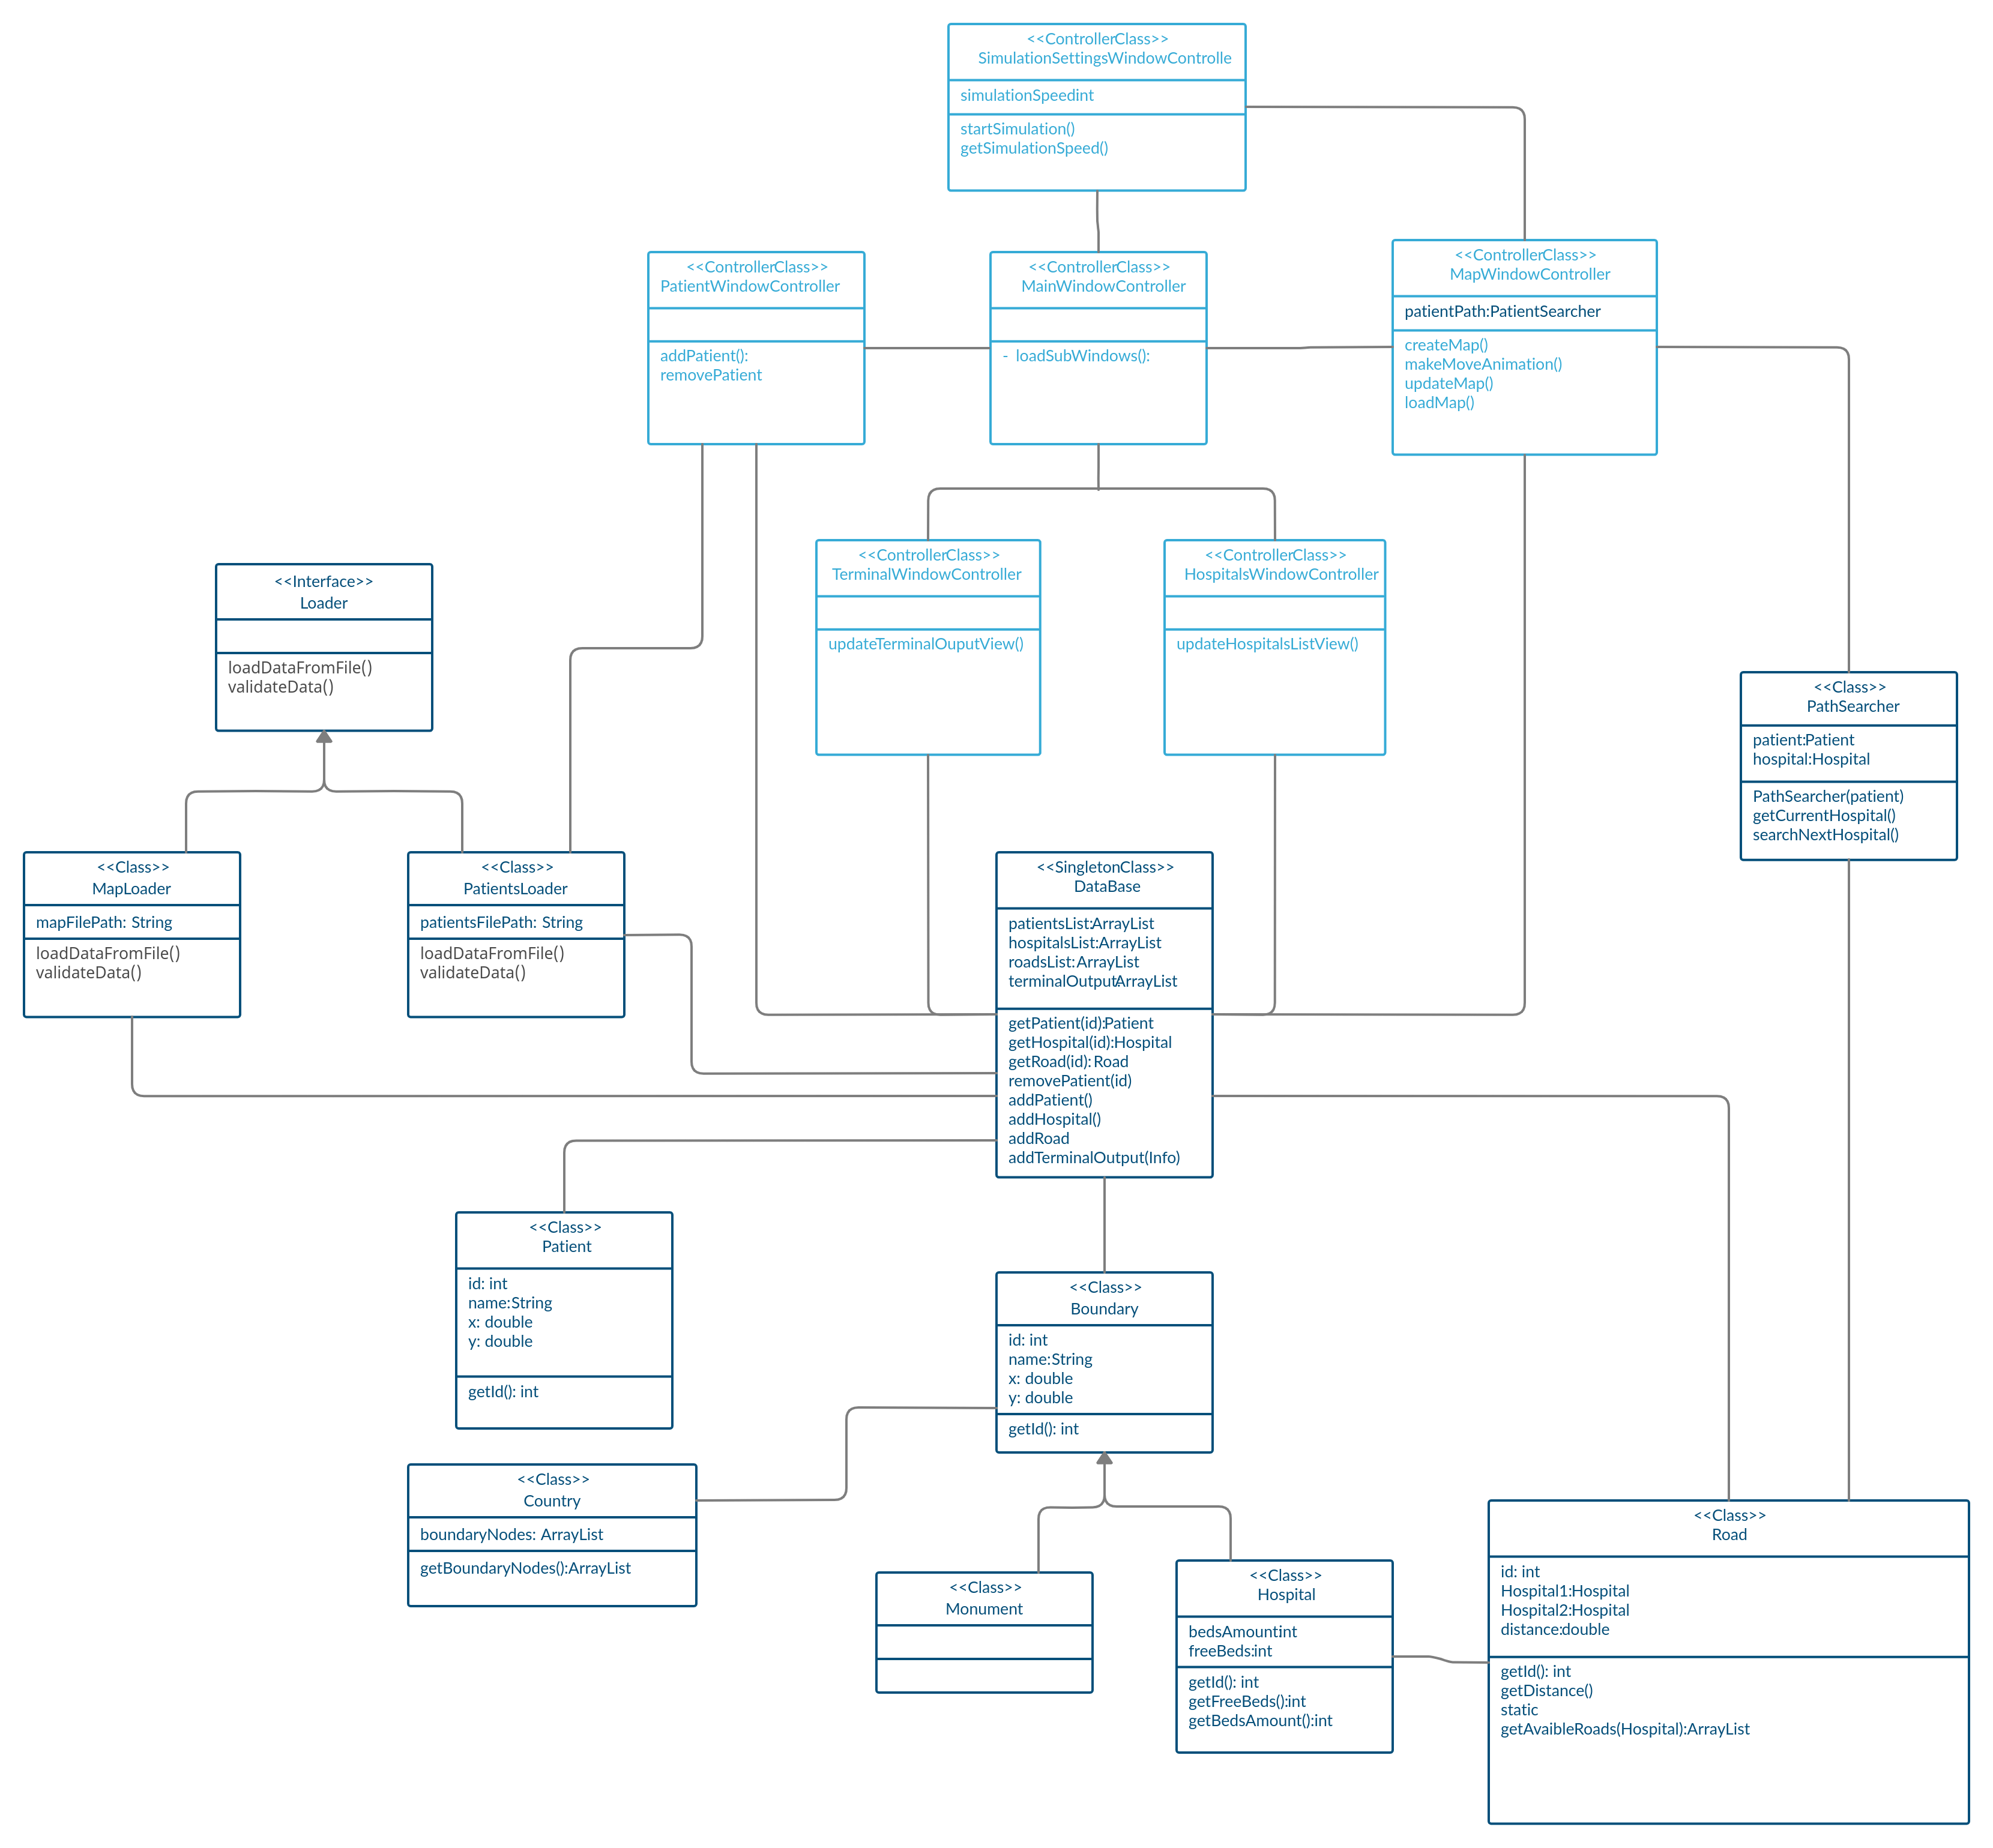
\includegraphics[width=\linewidth]{./images/diagram_klas.png}
  \caption{Diagram klas.}
  \label{fig:diagram_klas}
\end{figure}

Powyższy diagram prezentuje pomysł na zrealizowanie żądanej funkcjonalności.
W diagramie widoczne jest wyraźne rozdzielenie na klasy dotyczące reprezentacji graficznej oraz kodu, który wykonuje algorytmy.

Na samej górze, kolorem jasnoniebieskim zostały zaznaczone klasy kontrolerów okien JavyFX. Struktura opiera się na głównym oknie MainWindow, do którego następnie ładowane są kolejne okna.
Każde okno reprezentuje funkconalność okna przedstawioną w specyfikacji funkcjonalnej.

\begin{itemize}
    \item PatientWindowController - odpowiedzialny za dodawanie pacjentów do symulacji (ręcznie i z pliku)
    \item MapWindowController - odpowiedzialny za wyświetlenie mapy oraz operacje wizualizacyjne w symulacji. Wykorzystuje do swoich celów algorytm znajdujący kolejny szpital, do którego musi zostać przesłany pacjent.
    \item TerminalWindowController - odpowiedzialny za przetrzymywanie i pokazywanie komunikatów programu.
    \item HospitalsWindowController - odpowiedzialny za reprezentację stanu każdego szpitala i pokazywanie ich zmian.
    \item SimulationSettingsWindowController - odpowiedzialny za wskazanie parametrów symulacji np. prędkość jej postępowania.
    \item MainWindowController - główne okno programu. Zarządza wszystkimi pozostałymi oknami oraz przekazuje referencje i zmiany stanów pomiędzy oknami.
\end{itemize}
W dolnej części diagramu przedstawione zostały wyszczególnione klasy związane z wykonywaniem algorytmów.
Głównym ich zadaniem jest realizacja funkcjonalności projektu.
Można je podzielić na klasy reprezentujące dane oraz funkcjonalności programu.
Klasy reprezentujące dane:

\begin{itemize}
    \item Patient - klasa reprezentująca pacjenta. Posiada współrzędne kartezjańske, identyfikator oraz nazwę.
    \item Road - klasa reprezentująca połączenia między szpitalami. Wyposażona w referencje do szpitali, do których jest w stanie doprowadzić, identyfikator oraz czas, potrzebny na jej pokonanie.
    \item Boundary - klasa reprezentująca obiekty wchodzące w skład granicy pańśtwa. Zawiera współrzędne kartezjańskie, identyfikator oraz nazwę.
    \item Hospital - klasa reprezentująca szpital, pochodna Boundary, ponieważ może wyznaczać granicę państwa. Posiada dodatkowo informację o ilości wszystkich i wolnych łóżek w szpitalu.
    \item Monument - klasa reprezentująca pomnik. Stworzona w celu odróżnienia szpitala od pomnika.
    \item Country - klasa reprezentująca państwo. Zawiera listę obiektów, które wyznaczają granice państwa.

\end{itemize}


Poniżej zostały przedstawione klasy odpowiedzialne za operacje algorytmiczne:

\begin{itemize}
    \item DataBase - klasa przetrzymująca dane. Jest to klasa singleton, która będzie dostarczała dane do wszystkich klas. Taka realizacja pozwoli na spójny dostęp do danych.
    \item PathSearcher - klasa znajdująca szpitale, do których będziemy chcieli przewozić pacjentów. Jej wynik będzie dostarczany do kontrolerów okien w celu aktualizacji postępu symulacji.
    \item Interfejs Loader - interfejs ujednolicający sposób tworzenia pacjentów oraz mapy z listy. Pozwoli na generyczne pobieranie danych z plików i zapewni zdolności uogólniające kodu.
    \item MapLoader - klasa implementująca interfejs Loader. Głównym zadaniem jest wczytanie mapy z pliku.
    \item MapLoader - klasa implementująca interfejs Loader. Głównym zadaniem jest wczytanie pacjentów z pliku.
\end{itemize}

Takie zaprojektowanie systemu pozwoli na oddzielenie warstwy kontroli okien od warstwy obliczeniowej.
Dodatkowo powstały interfejs pozwoli na zwiększenie uogólnienia zastosowania kodu i ograniczenie powielania kodu.
Dziedzieczenie obiektów, pozwoli na łatwiejsze sprawdzenie granic państwa, bez rozróżnienia, czy obiekt jest szpitalem czy pomnikiem.

\section{Problemy Algorytmiczne}

Całe zadanie symulacji transportu pacjenta do szpitali można rozbić na pomniejsze problemy.
Rozwiązując je sekwencyjnie uzyskać można rzeczywiste rozwiązanie problemu przewozu pacjentów przy pomocy karetek do szpitali.
Poniżej znajdują się opisy wydzielonych problemów programistycznych, których rozwiązanie pozwoli na otrzymanie końcowego wyniku.

\subsection{Przedstawienie mapy państwa}

Pierwszym krokiem programu jest wczytanie środowiska, w którym należy rozwiązać symulację.
Granice państwa muszą być figurą wypukłą opartą na najbardziej zewnętrznych punktach.
Mimo tego nie wszystkie zewnętrzne punkty wyznaczają granice pańśtwa, ponieważ połączenie niektórych z nich powoduje powstanie bryły niewypukłej.

W tym celu zastosowany zostanie poniższy algorytm bazujący na problemie "Convex Hull" w implementacji opracowanej przez jednego z członków zespołu.
Wierzchołkami przedstawionego poniżej grafu są szpitale oraz pomniki, których jedyna funkcja to poszerzenie granic państwa.
Poniżej znajduje się opis algorytmu:

\begin{enumerate}
    \item Szukaj wierzchołka o najmniejszej współrzędnej x.
    \item Dodaj go do nowo utworzonej listy wierzchołków.
    \item Stwórz początkowo pustą listę współczynników kierunkowych, która będzie gromadzić nachylenie prostej przechodzącej przez wybrane dwa wierchołki grafu.
    \item Szukaj kolejnego wierzchołka o najmniejszej możliwej współrzędnej x (może to być również wierchołek, który ma taką samą współrzędną w osi x o ile ma większą wartość w osi y).
    \item Po znalezieniu wierzhołka wyznacz współczynnik kierunkowy prostej łączącej go i poprzedni punkt. Jeśli jest on mniejszy od ostatniego elemtnu na liście współczynników to dodaj ten wierzchołek do listy wierzchołków, a współczynnik do listy współczynników. Jeśli lista współczynników jest pusta to warunek jest zawsze spełniony. Jeżeli warunek nie jest sepłniony to usuń z obu list ostatni element i sprawdź analogiczny warunek dla nowych ostatnich elementów obu list. Jeśli warunek jest spełniony to dodaj elementy do listy, jeśli nie to ponownie usuwaj tak długo aż warunek będzie spełniony.
    \item Kroki od 3 do 5 powtarzaj tak długo aż zostaną sprawdzone wszystkie wierzchołki - czy nie ma nowego wierzchołka o współrzędnej y większej niż ostatni z listy.
    \item Wykonaj kroki 1-6 z tym, że:
    \begin{enumerate}[a)]
        \item zacznij od ostatniego punktu z listy wierzchołków z punktów 1-6,
        \item szukaj kolejnych wierzchołków malejąco wzdłuż osi y takich, żeby ich współrzędne x były coraz większe,
        \item postępuj analogicznie jak w punkcie 5.
    \end{enumerate}
    \item Wykonaj kroki 1-6 z tym, że:
    \begin{enumerate}[a)]
        \item zacznij od ostatniego punktu z listy wierchołków z punktu 7,
        \item szukaj kolejnych wierzchołków malejąco wzdłuż osi x takich, żeby ich współrzędne y były coraz mniejsze,
        \item postępuj jak w punkcie 5.
    \end{enumerate}
    \item Wykonaj kroki 1-6 z tym, że:
    \begin{enumerate}[a)]
        \item zacznij od ostatniego punktu z listy wierzchołków z punktu 8,
        \item szukaj kolejnych wierzchołków rosnąco wzdłuż osi y takich, żeby ich współrzędne x były coraz mniejsze,
        \item postępuj analogicznie jak w punkcie 5.
    \end{enumerate}
\end{enumerate}

\subsection{Znalezienie skrzyżowań}

W postawionym zadaniu istnieje założenie, że jeżeli drogi przecinają się to w miejscu przecięcia powstaje skrzyżowanie.
Powoduje to, że od pewnego szpitala do innego szpitala można dojechać okrężną, lecz szybszą drogą, mimo że nie istnieje ona w pliku wejściowym.
Biorąc pod uwagę, że wszystkie obiekty mapy posiadają współrzędne kartezjańskie, punkty przecięć można wyznaczyć w sposób czysto matematyczny.
Przedstawiając drogę od szpitala do szpitala jako odcinek, można przedstawić wszystkie drogi jako odcinki i znaleźć ich punkty przecięcia.
Jest to metoda naiwna, ponieważ wymaga ona przeanalizowania każdej drogi z każdą inną drogą ze zbioru dróg.
O ile dla jednej pary złożoność obliczeniowa to O(1), tak dla n dróg jest to już O($n^2$).

Istnieje także bardziej przemyślany algorytm, który poprzez "omiecenie wiązką" przez wszystkie odcinki jest w stanie wykryć ich punkty przecięć.
Implementacja algorytmu Bentley–Ottmann wymaga przedstawienia dróg jako posortowanych punktów względem osi X oraz odcinków. Algorytm można przedstawić następująco:
\begin{itemize}
    \item Pionowa linia "przemiata" wszystkie punkty od lewej do prawej.
    \item Po natknięciu się na lewy(początkowy) punkt odcinka, odcinek oznaczany jest jako aktywny.
    \item Następnie sprawdzane są przecięcia z najbliższymi, aktywnymi odcinkami powyżej i poniżej aktualnego odcinka.
    \item Jeżeli odcinki aktywne się przecinają wtedy jest znajdowany i zapamiętywany punkt przecięcia między tymi odcinkami.
    \item W momencie gdy pionowa linia napotka końcowy punkt odcinka, wtedy dezaktywuje ona odcinek. Sprawia to, że odcinek nie jest brany dalej do analizy przecięć z innymi odcinkami.
\end{itemize}
Taki sposób pozwala na ograniczenie zbioru sprawdzanych odcinków do sąsiedztwa potencjalnie przecinających się odcinków.
Dzięki temu nie trzeba sprawdzać każdej pary odcinków ze sobą, co skutkuje złożonością obliczeniową rzędu O((n+k)log n), gdzie n to liczba odcinków, a k liczba przecięć.

Rozwijając ten algorytm, punkty przecięć zostaną skrzyżowaniami z punktu widzenia działania programu, a drogi na przecięciach zostaną zmodyfikowane w zależności od tego w jakiej proporcji punkt podzielił odcinki.


\subsection{Określenie czy pacjent znajduje się na terytorium państwa}

Założeniem projektu jest obsługa pacjentów znajdujących się w obszarze państwa.
Jeżeli pacjent znajdujący się poza granicami państwa wymaga pomocy, wtedy karetka nie jest w stanie jej udzielić.
Algorytm wygląda następująco:

\begin{enumerate}
    \item Dla pacjenta o współrzędnych $(x_p,y_p)$ i każdego boku mapy państwa (wielokąta wypukłego) $M=\{W_1=(x_1,y_1), ..., W_n=(x_n,y_n)\}$, oblicz i sprawdź znak:
    $$h=(y_{i+1}-y_i)*(x_p-x_i)-(x_{i+1}-x_i)*(y_p-y_i)$$
    \item Jeśli $h$ dla wszystkich boków mapy ma taki sam znak, to pacjent znajduje się na terytorium państwa. Jeśli nie, to pacjent znajduje się poza granicami państwa.
\end{enumerate}

\subsection{Transport pacjenta do najbliższego szpitala}

Transport pacjenta jest to szereg operacji mających na celu doprowadzić pacjenta do szpitala, w którym może zostać mu udzielona pomoc.
Składa się on z operacji przewiezienia pacjenta do najbliższego szpitala, a jeżeli nie będzie w nim miejsca, znalezienie takiego szpitala , który jest w stanie tą pomoc zaoferować.
Poszukiwanie szpitali odbywa się poprzez przewożenia pacjenta do szpitala i dopiero sprawdzania czy są w nim miejsca.
Algorytm dostarczenia pacjenta do placówki prezentuje się następująco:

\begin{enumerate}
    \item Oblicz odległość pacjenta do wszystkich szpitali wg wzoru:
    $$d_i=\sqrt{({x_s}_i-x_p)^2+({y_s}_i-y_p)^2}$$
    \item Wybierz szpital, do którego odległość $d$ jest najmniejsza
    \item Udaj się do wybranego szpitala i po dojeździe (gdy pozycja pacjenta=pozycji szpitala) sprawdź czy w wybranym szpitalu jest wolne łóżko. Jeśli TAK – KONIEC transportu pacjenta, zostaw pacjenta w szpitalu. Jeśli NIE - oznacz szpital jako odwiedzony i przejdź do punktu 4.
    \item Dla szpitala, w którym obecnie znajduje się pacjent wyznacz inny szpital, do którego droga jest najkrótsza:
    \begin{enumerate}[4.1.]
        \item Dla każdego szpitala i wierzchołka bezpośrednio połączonego z obecnym szpitalem (skrzyżowania) wyznacz długości połączeń i zapamiętaj je.
        \item Zawsze jeśli sprawdziłeś już jakiś wierzchołek zapamiętaj ten fakt (zapamiętaj, że udało się do niego wyznaczyć jakąkolwiek drogę).
        \item Jeśli w danym szpitalu nie było jeszcze karetki, to zakończ przeszukiwanie ścieżek przechodzących przez ten szpital.
        \item Jeśli w danym miejscu była już karetka, to przeszukuj dalej graf, zapamiętując sumaryczną drogę i trasę do każdego wierzchołka.
        \item Kończ przeszukiwanie danej ścieżki, gdy dotrzesz do wierzchołka, który był już sprawdzony.
        \item Po przeszukaniu całego grafu z obecnego szpitala, wybierz nieodwiedzony szpital, do ktorego sumaryczna droga jest najkrótsza. Z tak wybranym szpitalem przejdź do punktu 3. 
    \end{enumerate}
\end{enumerate}

\section{Testy oprogramowania}

Do testowania oprogramowania użyte będzie narzędzie JUnit.

Dla plików wejściowych - pliku z mapą oraz pliku z pacjentami przeprowadzone zostaną następujące testy:
 
\begin{enumerate}
    \item Pusty plik.
    \item Pusta sekcja.
    \item Brak tytułu sekcji (znaku "\#").
    \item Nieprawidłowa liczba znaków strumienia "\textbar".
    \item Nieprawidłowy typ danych.
    \item Niepoprawne watości danych - niedopuszczalna wartość zerowa, ujemnna lub wartość spoza zakresu danego typu danych.
    \item Powtarzające się id lub para id (sekcja "Drogi").
    \item Wykorzystanie nieistniejącego id szpitala w sekcji "Drogi".
\end{enumerate}

Inne (niedotyczące plików wejściowych) testy programu:
\begin{enumerate}
    \item
\end{enumerate}


\section{Źródła}

\begin{enumerate}[{[1]}]
    \item \url{http://0x80.pl/articles/point_in_polygon.html} \\(data i godzina dostępu: 16.12.2020 21:39)
    \item \url{https://eduinf.waw.pl/inf/utils/011_2011/0105.php} \\(data i godzina dostępu: 17.12.2020 15:21)
    \item \url{https://www.geeksforgeeks.org/convex-hull-set-2-graham-scan/?ref=lbp} \\(data i godzina dostępu: 17.12.2020 16:52)
\end{enumerate}

\end{document}{article}


